\section{Construction and the motivating execution}
\label{sec:construction}

\qperiapt{} combines ML-KEM-768 and X25519 in its ContextBound hybrid KEM
and authenticates protocol controls with an ML-DSA-65/P-256 identity.
Our analysis follows the persistent session and rekey machinery: an original
operation first reserves its entropy, places the resulting token in a retained
plan, and later computes or replays the corresponding KEM operation. An exact
retry uses the same reservation. The protocol alternates the proposing endpoint
across epochs and carries separate send, receive, and confirmed-epoch state.

\paragraph{Fixed cryptographic context.}
The combiner hashes a length-delimited encoding of the two component secrets,
both public keys and ciphertexts, and domain, suite, policy and
application-context fields. On the rekey path, the application context is a
domain-separated digest of the complete retained offer wire and is nested
with the admitted policy digest. These fields form fixed inputs of the
original operation; exact replay retains that binding and its reserved tape.
The source correspondence in Appendix~\ref{app:contextbound-source} identifies
the encoding and reservation constructors used here.

\subsection{Reservations and persistent representations}

A generation reservation determines the future hybrid key pair. An encapsulation
reservation, together with the authenticated offer, determines the corresponding
ciphertext and contribution. The implementation seals these reservations under
the host wrapping key. It persists the selected target in a pending write before
installing that target as the next journal image. Applying or reopening that
write preserves its original contents.

A journal image aggregates state from multiple sessions. Updating a sibling
session advances the global image revision and samples a new outer encryption
nonce, while the target session's retained reservation can remain unchanged.
Consequently, the journal revision, outer nonce, local operation identifier,
and original entropy reservation represent distinct identities. We preserve
these distinctions in the model and relate them to the native execution boundaries.

\begin{table}[t]
\centering
\small
\begin{tabularx}{\linewidth}{@{}lXX@{}}
\toprule
Event & Effect on the target operation & Provenance fact \\
\midrule
Reserve & Draw KEM entropy and seal its replay token & Creates an original source \\
Persist target & Retain the original pending-write bytes & Creates an acquisition opportunity \\
Apply or retry & Install or replay the retained target & Preserves the source \\
Sibling write & Re-encode the aggregate journal with a new outer nonce & Preserves unchanged target sources \\
Confirm & Advance the relevant endpoint's protocol state & Records protocol progress \\
\bottomrule
\end{tabularx}
\caption{The events tracked by the analysis. Several events may occur in one
symbolic transition; the native execution exposes their separate boundaries.}
\label{tab:events}
\end{table}

\subsection{Root and traffic dependencies}

Write $R_{e-1}$ for the preceding root, $S_e$ for the hybrid contribution,
$C_e$ for the public response core, and $O_e,P_e$ for the complete signed
offer and response. With the construction's canonical encodings and
domain-separated transcript hashes, its dependency equations are
\begin{align}
R_e &=
 \operatorname{HKDF}_{\rm SHA256}
 \bigl(R_{e-1},S_e,d_R\Vert H(d_C,C_e),32\bigr), \label{eq:root}\\
T_e &=
 \operatorname{HKDF}_{\rm SHA256}
 \bigl(\mathit{sid},R_e,
 d_T\Vert\mathit{ctx}\Vert e\Vert H(d_{\rm tr},O_e\Vert P_e),128\bigr).
 \label{eq:traffic}
\end{align}
Here HKDF arguments denote salt, input key material, information, and output
length in bytes. $T_e$ supplies two directional traffic chains and two
acknowledgement keys. The actual domain strings and encodings are pinned by the
source locations in Appendix~\ref{app:artifacts}.

These equations describe a concrete derivation path. A captured generation
reservation and matching wrapping key reconstruct the private key; a subsequent
public ciphertext then yields $S_e$. A captured encapsulation reservation yields
the same contribution using its retained offer. Combining $S_e$ with a disclosed
$R_{e-1}$ and the public control wires reproduces $R_e$ and the traffic material.
Honest admission checks can still reject an operation inside the SDK while an
adversary holding these inputs performs the underlying computation independently.

\subsection{Asynchronous confirmation and a later exposed epoch}

Consider the native execution in Figure~\ref{fig:delayed-receipt}. Endpoint $B$
commits the first receipt, advances locally, and prepares an epoch-two offer
before $A$ receives that receipt. At the capture point their local observations
are
\[
 A:(c,s,r,p)=(0,1,0,1),\qquad
 B:(c,s,r,p)=(1,1,1,2),
\]
where $c,s,r$ are confirmed, send, and receive epochs, and $p$ is the pending
target epoch. The snapshot of $B$ contains $R_1$ and the original generation
reservation for epoch two. After delivery resumes, those captured inputs and
the public exchange reconstruct epoch-two traffic.

\begin{figure}[t]
\centering
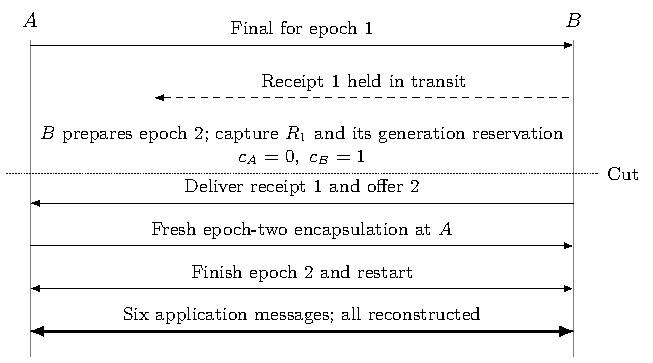
\includegraphics[width=\linewidth]{figures/confirmation-cut.pdf}
\caption{A retained native disclosure execution. The smaller confirmed counter
is zero at capture, while the captured reservation enables epoch-two traffic
recovery after the public exchange. The dotted Cut orders the exposure and the subsequent
fresh encapsulation; it does not refresh the earlier generation reservation.}
\label{fig:delayed-receipt}
\end{figure}

The resulting counterexample targets the proposed bound
$\min(c_A,c_B)+1$: its value is one, yet epoch-two traffic is exposed.
The protocol's asymmetric progress is legitimate. Recovery reasoning must
therefore follow the retained inputs and their descendants rather than identify
the two endpoints' confirmation counters.

